\question{}

พิซซ่าถาดหนึ่งถูกตัดแบ่งด้วยรัศมีออกเป็นพิซซ่าชิ้นย่อย ๆ 8 ชิ้นที่มาขนาดเท่า ๆ กัน\;
ต่อจากนั้นพิซซ่า\uline{แต่ละชิ้น}ย่อยทุกชิ้นจะถูกทาด้วยซอส 1 ใน 3 ชนิด (ได้แก่ ซอสขาว ซอสแดง หรือซอสน้ำตาล)

\medskip\noindent
\textbf{\uline{นิยาม}} พิซซ่าสองถาดจะมีหน้าตา\uline{แบบเดียวกัน} 
ก็ต่อเมื่อ หากสามารถหมุนถาดพิซซ่าถาดหนึ่งให้มีหน้าตาเหมือนกันพิซซ่าอีกถาดหนึ่งได้

\begin{fullwidth}
    \begin{multicols}{2}
        \begin{center}
            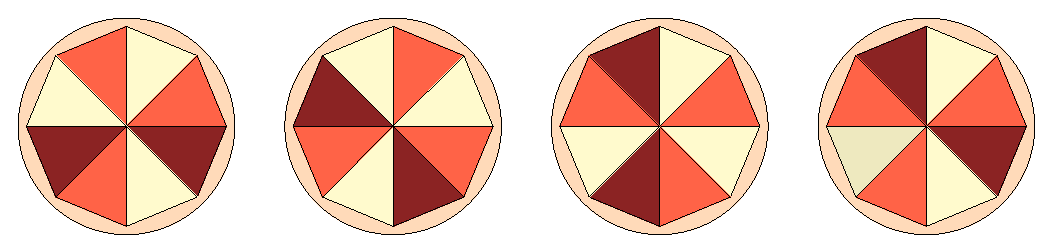
\includegraphics[width=0.85\linewidth]{figures/ponder_central_regional_pizzapaint_01.eps}\\
            ตัวอย่างของพิซซ่าที่หน้าตา\uline{เหมือนกัน}        
            
            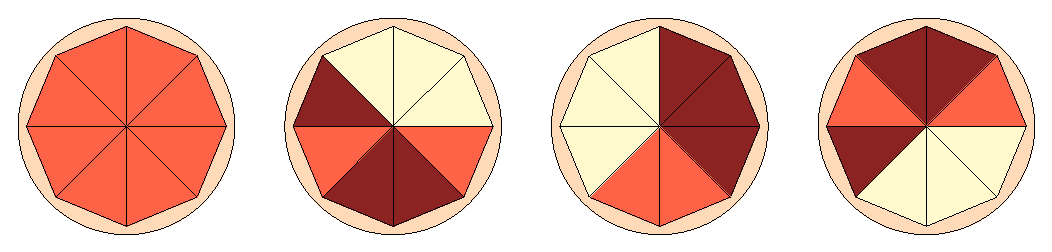
\includegraphics[width=0.85\linewidth]{figures/ponder_central_regional_pizzapaint_02.eps}\\
            ตัวอย่างของพิซซ่าที่หน้าตา\uline{แตกต่างกันทั้งหมด}
        \end{center}
        
    \end{multicols}
\end{fullwidth}

\medskip\noindent
\textbf{\uline{โจทย์}} อยากทราบว่าเราจะได้ถาดพิซซ่าที่หน้าตามีการทาซอสออกมาแตกต่างกันทั้งหมดกี่แบบ?

